\documentclass[a4paper,11pt,twoside]{article}
%\documentclass[a4paper,11pt,twoside,se]{article}

\usepackage{UmUStudentReport}
\usepackage{verbatim}   % Multi-line comments using \begin{comment}
\usepackage{courier}    % Nicer fonts are used. (not necessary)
\usepackage{pslatex}    % Also nicer fonts. (not necessary)
\usepackage[pdftex]{graphicx}   % allows including pdf figures
\usepackage{listings}
\usepackage{pgf-umlcd}
%\usepackage{lmodern}   % Optional fonts. (not necessary)
%\usepackage{tabularx}
%\usepackage{microtype} % Provides some typographic improvements over default settings
%\usepackage{placeins}  % For aligning images with \FloatBarrier
%\usepackage{booktabs}  % For nice-looking tables
%\usepackage{titlesec}  % More granular control of sections.

% DOCUMENT INFO
% =============
\department{Department of Computing Science}
\coursename{Object-Oriented Programming Methodology 7.5 p}
\coursecode{5DV133}
\title{OU1 Clock}
\author{Lorenz Gerber ({\tt{dv15lgr@cs.umu.se}} {\tt{lozger03@student.umu.se}})}
\date{2016-04-07}
%\revisiondate{2016-01-18}
\instructor{Anders Broberg / Niklas Fries / Adam Dahlgren / Jonathan
  Westin / Erik Moström / Alexander Sutherland}


% DOCUMENT SETTINGS
% =================
\bibliographystyle{plain}
%\bibliographystyle{ieee}
\pagestyle{fancy}
\raggedbottom
\setcounter{secnumdepth}{2}
\setcounter{tocdepth}{2}
%\graphicspath{{images/}}   %Path for images

\usepackage{float}
\floatstyle{ruled}
\newfloat{listing}{thp}{lop}
\floatname{listing}{Listing}



% DEFINES
% =======
%\newcommand{\mycommand}{<latex code>}

% DOCUMENT
% ========
\begin{document}
\lstset{language=C}
\maketitle
\thispagestyle{empty}
\newpage
\tableofcontents
\thispagestyle{empty}
\newpage

\clearpage
\pagenumbering{arabic}

\section{Introduction} 
Aim of this laboration was to implement a digital clock and an alarm
clock in the object oriented language Java. The class design was
mostly defined in the assignment. After implementing \textit{Clock}
and \textit{Alarm} classes, a \textit{main} method had to be written
to provide test cases of the implemented classes. Additionally, it was
recommended to also write JUnit tests for all classes. 

\section{Usage Instructions}
The files provided in an zip archieve are: \textit{ClockApp.java,
  Clock.java, ClockTest.java, NumberDisplay.java,
  NumberDisplayTest.java, Alarm.java, AlarmTest.java}. To build from
the command line, \textit{javac ClockApp.java} is invoked. To run the
program \textit{java ClockApp}.

The program does not take any input and does not produce any
output. During runtime, it writes several lines to standard out. The
implications of the printout will be described further in the section 
\textit{testing}.

\section{System Description}
class diagram, Class Responsibility and Collaborators, programflow

\section{Testing}




\begin{figure}
  \centering
  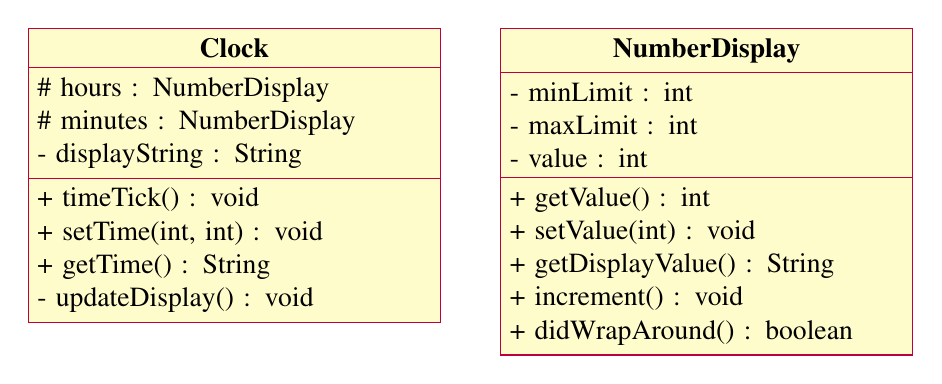
\begin{tikzpicture}
    \begin{class}[text width = 5cm]{Clock}{0,0}
      \attribute{\# hours : NumberDisplay}
      \attribute{\# minutes : NumberDisplay}
      \attribute{- displayString : String}

      \operation{+ timeTick() : void}
      \operation{+ setTime(int, int) : void} 
      \operation{+ getTime() : String}
      \operation{- updateDisplay() : void}
    \end{class}

    \begin{class}[text width = 5cm]{NumberDisplay}{6, 0}
      \attribute{- minLimit : int}
      \attribute{- maxLimit : int}
      \attribute{- value : int}

      \operation{+ getValue() : int}
      \operation{+ setValue(int) : void}
      \operation{+ getDisplayValue() : String}
      \operation{+ increment() : void}
      \operation{+ didWrapAround() : boolean}
    \end{class}
  \end{tikzpicture}
  \caption{\textit{Class diagrams of Clock and NumberDisplay.}}
  \label{fig:umlclass}  
\end{figure}


\section{Program Structure}

\section{Discussion}



\addcontentsline{toc}{section}{\refname}
\bibliography{references}

\end{document}
